\documentclass[11pt,a4paper]{article}

    \usepackage{indentfirst}
    \usepackage{listings}
    \usepackage{float}
    \usepackage[T1]{fontenc}
    % Nicer default font (+ math font) than Computer Modern for most use cases
    \usepackage{mathpazo}

    % Basic figure setup, for now with no caption control since it's done
    % automatically by Pandoc (which extracts ![](path) syntax from Markdown).
    \usepackage{graphicx}
    % We will generate all images so they have a width \maxwidth. This means
    % that they will get their normal width if they fit onto the page, but
    % are scaled down if they would overflow the margins.
    \graphicspath{ {./img/} }
    \makeatletter
    \def\maxwidth{\ifdim\Gin@nat@width>\linewidth\linewidth
    \else\Gin@nat@width\fi}
    \makeatother
    \let\Oldincludegraphics\includegraphics
    % Set max figure width to be 80% of text width, for now hardcoded.
    \renewcommand{\includegraphics}[1]{\Oldincludegraphics[width=.8\maxwidth]{#1}}
    % Ensure that by default, figures have no caption (until we provide a
    % proper Figure object with a Caption API and a way to capture that
    % in the conversion process - todo).
    \usepackage{caption}
    \DeclareCaptionLabelFormat{nolabel}{}
    \captionsetup{labelformat=nolabel}

    \usepackage{adjustbox} % Used to constrain images to a maximum size
    \usepackage{xcolor} % Allow colors to be defined
    \usepackage{enumerate} % Needed for markdown enumerations to work
    \usepackage{geometry} % Used to adjust the document margins
    \usepackage{amsmath} % Equations
    \usepackage{amssymb} % Equations
    \usepackage{textcomp} % defines textquotesingle
    % Hack from http://tex.stackexchange.com/a/47451/13684:
    \AtBeginDocument{%
        \def\PYZsq{\textquotesingle}% Upright quotes in Pygmentized code
    }
    \usepackage{upquote} % Upright quotes for verbatim code
    \usepackage{eurosym} % defines \euro
    \usepackage[mathletters]{ucs} % Extended unicode (utf-8) support
    \usepackage[utf8x]{inputenc} % Allow utf-8 characters in the tex document
    \usepackage{fancyvrb} % verbatim replacement that allows latex
    \usepackage{grffile} % extends the file name processing of package graphics
                         % to support a larger range
    % The hyperref package gives us a pdf with properly built
    % internal navigation ('pdf bookmarks' for the table of contents,
    % internal cross-reference links, web links for URLs, etc.)
    \usepackage{hyperref}
    \usepackage{longtable} % longtable support required by pandoc >1.10
    \usepackage{booktabs}  % table support for pandoc > 1.12.2
    \usepackage[inline]{enumitem} % IRkernel/repr support (it uses the enumerate* environment)
    \usepackage[normalem]{ulem} % ulem is needed to support strikethroughs (\sout)
                                % normalem makes italics be italics, not underlines

    % Colors for the hyperref package
    \definecolor{urlcolor}{rgb}{0,.145,.698}
    \definecolor{linkcolor}{rgb}{.71,0.21,0.01}
    \definecolor{citecolor}{rgb}{.12,.54,.11}

    % ANSI colors
    \definecolor{ansi-black}{HTML}{3E424D}
    \definecolor{ansi-black-intense}{HTML}{282C36}
    \definecolor{ansi-red}{HTML}{E75C58}
    \definecolor{ansi-red-intense}{HTML}{B22B31}
    \definecolor{ansi-green}{HTML}{00A250}
    \definecolor{ansi-green-intense}{HTML}{007427}
    \definecolor{ansi-yellow}{HTML}{DDB62B}
    \definecolor{ansi-yellow-intense}{HTML}{B27D12}
    \definecolor{ansi-blue}{HTML}{208FFB}
    \definecolor{ansi-blue-intense}{HTML}{0065CA}
    \definecolor{ansi-magenta}{HTML}{D160C4}
    \definecolor{ansi-magenta-intense}{HTML}{A03196}
    \definecolor{ansi-cyan}{HTML}{60C6C8}
    \definecolor{ansi-cyan-intense}{HTML}{258F8F}
    \definecolor{ansi-white}{HTML}{C5C1B4}
    \definecolor{ansi-white-intense}{HTML}{A1A6B2}

    % Colors for the Highlighting
    \definecolor{hlgreen}{rgb}{0,0.6,0}
    \definecolor{hlgray}{rgb}{0.5,0.5,0.5}
    \definecolor{hlmauve}{rgb}{0.58,0,0.82}

    % Defining the Highlighting
    \lstset{
        backgroundcolor=\color{white},
        basicstyle=\footnotesize,
        breaklines=true,
        captionpos=b,
        commentstyle=\color{hlgreen},
        escapeinside={\%*}{*)},
        keywordstyle=\color{blue},
        stringstyle=\color{hlmauve},
        frame=single
    }
    % commands and environments needed by pandoc snippets
    % extracted from the output of `pandoc -s`
    \providecommand{\tightlist}{%
      \setlength{\itemsep}{0pt}\setlength{\parskip}{0pt}}
    \DefineVerbatimEnvironment{Highlighting}{Verbatim}{commandchars=\\\{\}}
    % Add ',fontsize=\small' for more characters per line
    \newenvironment{Shaded}{}{}
    \newcommand{\KeywordTok}[1]{\textcolor[rgb]{0.00,0.44,0.13}{\textbf{{#1}}}}
    \newcommand{\DataTypeTok}[1]{\textcolor[rgb]{0.56,0.13,0.00}{{#1}}}
    \newcommand{\DecValTok}[1]{\textcolor[rgb]{0.25,0.63,0.44}{{#1}}}
    \newcommand{\BaseNTok}[1]{\textcolor[rgb]{0.25,0.63,0.44}{{#1}}}
    \newcommand{\FloatTok}[1]{\textcolor[rgb]{0.25,0.63,0.44}{{#1}}}
    \newcommand{\CharTok}[1]{\textcolor[rgb]{0.25,0.44,0.63}{{#1}}}
    \newcommand{\StringTok}[1]{\textcolor[rgb]{0.25,0.44,0.63}{{#1}}}
    \newcommand{\CommentTok}[1]{\textcolor[rgb]{0.38,0.63,0.69}{\textit{{#1}}}}
    \newcommand{\OtherTok}[1]{\textcolor[rgb]{0.00,0.44,0.13}{{#1}}}
    \newcommand{\AlertTok}[1]{\textcolor[rgb]{1.00,0.00,0.00}{\textbf{{#1}}}}
    \newcommand{\FunctionTok}[1]{\textcolor[rgb]{0.02,0.16,0.49}{{#1}}}
    \newcommand{\RegionMarkerTok}[1]{{#1}}
    \newcommand{\ErrorTok}[1]{\textcolor[rgb]{1.00,0.00,0.00}{\textbf{{#1}}}}
    \newcommand{\NormalTok}[1]{{#1}}

    % Additional commands for more recent versions of Pandoc
    \newcommand{\ConstantTok}[1]{\textcolor[rgb]{0.53,0.00,0.00}{{#1}}}
    \newcommand{\SpecialCharTok}[1]{\textcolor[rgb]{0.25,0.44,0.63}{{#1}}}
    \newcommand{\VerbatimStringTok}[1]{\textcolor[rgb]{0.25,0.44,0.63}{{#1}}}
    \newcommand{\SpecialStringTok}[1]{\textcolor[rgb]{0.73,0.40,0.53}{{#1}}}
    \newcommand{\ImportTok}[1]{{#1}}
    \newcommand{\DocumentationTok}[1]{\textcolor[rgb]{0.73,0.13,0.13}{\textit{{#1}}}}
    \newcommand{\AnnotationTok}[1]{\textcolor[rgb]{0.38,0.63,0.69}{\textbf{\textit{{#1}}}}}
    \newcommand{\CommentVarTok}[1]{\textcolor[rgb]{0.38,0.63,0.69}{\textbf{\textit{{#1}}}}}
    \newcommand{\VariableTok}[1]{\textcolor[rgb]{0.10,0.09,0.49}{{#1}}}
    \newcommand{\ControlFlowTok}[1]{\textcolor[rgb]{0.00,0.44,0.13}{\textbf{{#1}}}}
    \newcommand{\OperatorTok}[1]{\textcolor[rgb]{0.40,0.40,0.40}{{#1}}}
    \newcommand{\BuiltInTok}[1]{{#1}}
    \newcommand{\ExtensionTok}[1]{{#1}}
    \newcommand{\PreprocessorTok}[1]{\textcolor[rgb]{0.74,0.48,0.00}{{#1}}}
    \newcommand{\AttributeTok}[1]{\textcolor[rgb]{0.49,0.56,0.16}{{#1}}}
    \newcommand{\InformationTok}[1]{\textcolor[rgb]{0.38,0.63,0.69}{\textbf{\textit{{#1}}}}}
    \newcommand{\WarningTok}[1]{\textcolor[rgb]{0.38,0.63,0.69}{\textbf{\textit{{#1}}}}}


    % Define a nice break command that doesn't care if a line doesn't already
    % exist.
    \def\br{\hspace*{\fill} \\* }
    % Math Jax compatability definitions
    \def\gt{>}
    \def\lt{<}
    % Document parameters
    \title{Relatório do Projeto}
    \author{Anderson R. Livramento e João V. Laitano}
    \date{Outubro 2018}

    % Pygments definitions

\makeatletter
\def\PY@reset{\let\PY@it=\relax \let\PY@bf=\relax%
    \let\PY@ul=\relax \let\PY@tc=\relax%
    \let\PY@bc=\relax \let\PY@ff=\relax}
\def\PY@tok#1{\csname PY@tok@#1\endcsname}
\def\PY@toks#1+{\ifx\relax#1\empty\else%
    \PY@tok{#1}\expandafter\PY@toks\fi}
\def\PY@do#1{\PY@bc{\PY@tc{\PY@ul{%
    \PY@it{\PY@bf{\PY@ff{#1}}}}}}}
\def\PY#1#2{\PY@reset\PY@toks#1+\relax+\PY@do{#2}}

\expandafter\def\csname PY@tok@w\endcsname{\def\PY@tc##1{\textcolor[rgb]{0.73,0.73,0.73}{##1}}}
\expandafter\def\csname PY@tok@c\endcsname{\let\PY@it=\textit\def\PY@tc##1{\textcolor[rgb]{0.25,0.50,0.50}{##1}}}
\expandafter\def\csname PY@tok@cp\endcsname{\def\PY@tc##1{\textcolor[rgb]{0.74,0.48,0.00}{##1}}}
\expandafter\def\csname PY@tok@k\endcsname{\let\PY@bf=\textbf\def\PY@tc##1{\textcolor[rgb]{0.00,0.50,0.00}{##1}}}
\expandafter\def\csname PY@tok@kp\endcsname{\def\PY@tc##1{\textcolor[rgb]{0.00,0.50,0.00}{##1}}}
\expandafter\def\csname PY@tok@kt\endcsname{\def\PY@tc##1{\textcolor[rgb]{0.69,0.00,0.25}{##1}}}
\expandafter\def\csname PY@tok@o\endcsname{\def\PY@tc##1{\textcolor[rgb]{0.40,0.40,0.40}{##1}}}
\expandafter\def\csname PY@tok@ow\endcsname{\let\PY@bf=\textbf\def\PY@tc##1{\textcolor[rgb]{0.67,0.13,1.00}{##1}}}
\expandafter\def\csname PY@tok@nb\endcsname{\def\PY@tc##1{\textcolor[rgb]{0.00,0.50,0.00}{##1}}}
\expandafter\def\csname PY@tok@nf\endcsname{\def\PY@tc##1{\textcolor[rgb]{0.00,0.00,1.00}{##1}}}
\expandafter\def\csname PY@tok@nc\endcsname{\let\PY@bf=\textbf\def\PY@tc##1{\textcolor[rgb]{0.00,0.00,1.00}{##1}}}
\expandafter\def\csname PY@tok@nn\endcsname{\let\PY@bf=\textbf\def\PY@tc##1{\textcolor[rgb]{0.00,0.00,1.00}{##1}}}
\expandafter\def\csname PY@tok@ne\endcsname{\let\PY@bf=\textbf\def\PY@tc##1{\textcolor[rgb]{0.82,0.25,0.23}{##1}}}
\expandafter\def\csname PY@tok@nv\endcsname{\def\PY@tc##1{\textcolor[rgb]{0.10,0.09,0.49}{##1}}}
\expandafter\def\csname PY@tok@no\endcsname{\def\PY@tc##1{\textcolor[rgb]{0.53,0.00,0.00}{##1}}}
\expandafter\def\csname PY@tok@nl\endcsname{\def\PY@tc##1{\textcolor[rgb]{0.63,0.63,0.00}{##1}}}
\expandafter\def\csname PY@tok@ni\endcsname{\let\PY@bf=\textbf\def\PY@tc##1{\textcolor[rgb]{0.60,0.60,0.60}{##1}}}
\expandafter\def\csname PY@tok@na\endcsname{\def\PY@tc##1{\textcolor[rgb]{0.49,0.56,0.16}{##1}}}
\expandafter\def\csname PY@tok@nt\endcsname{\let\PY@bf=\textbf\def\PY@tc##1{\textcolor[rgb]{0.00,0.50,0.00}{##1}}}
\expandafter\def\csname PY@tok@nd\endcsname{\def\PY@tc##1{\textcolor[rgb]{0.67,0.13,1.00}{##1}}}
\expandafter\def\csname PY@tok@s\endcsname{\def\PY@tc##1{\textcolor[rgb]{0.73,0.13,0.13}{##1}}}
\expandafter\def\csname PY@tok@sd\endcsname{\let\PY@it=\textit\def\PY@tc##1{\textcolor[rgb]{0.73,0.13,0.13}{##1}}}
\expandafter\def\csname PY@tok@si\endcsname{\let\PY@bf=\textbf\def\PY@tc##1{\textcolor[rgb]{0.73,0.40,0.53}{##1}}}
\expandafter\def\csname PY@tok@se\endcsname{\let\PY@bf=\textbf\def\PY@tc##1{\textcolor[rgb]{0.73,0.40,0.13}{##1}}}
\expandafter\def\csname PY@tok@sr\endcsname{\def\PY@tc##1{\textcolor[rgb]{0.73,0.40,0.53}{##1}}}
\expandafter\def\csname PY@tok@ss\endcsname{\def\PY@tc##1{\textcolor[rgb]{0.10,0.09,0.49}{##1}}}
\expandafter\def\csname PY@tok@sx\endcsname{\def\PY@tc##1{\textcolor[rgb]{0.00,0.50,0.00}{##1}}}
\expandafter\def\csname PY@tok@m\endcsname{\def\PY@tc##1{\textcolor[rgb]{0.40,0.40,0.40}{##1}}}
\expandafter\def\csname PY@tok@gh\endcsname{\let\PY@bf=\textbf\def\PY@tc##1{\textcolor[rgb]{0.00,0.00,0.50}{##1}}}
\expandafter\def\csname PY@tok@gu\endcsname{\let\PY@bf=\textbf\def\PY@tc##1{\textcolor[rgb]{0.50,0.00,0.50}{##1}}}
\expandafter\def\csname PY@tok@gd\endcsname{\def\PY@tc##1{\textcolor[rgb]{0.63,0.00,0.00}{##1}}}
\expandafter\def\csname PY@tok@gi\endcsname{\def\PY@tc##1{\textcolor[rgb]{0.00,0.63,0.00}{##1}}}
\expandafter\def\csname PY@tok@gr\endcsname{\def\PY@tc##1{\textcolor[rgb]{1.00,0.00,0.00}{##1}}}
\expandafter\def\csname PY@tok@ge\endcsname{\let\PY@it=\textit}
\expandafter\def\csname PY@tok@gs\endcsname{\let\PY@bf=\textbf}
\expandafter\def\csname PY@tok@gp\endcsname{\let\PY@bf=\textbf\def\PY@tc##1{\textcolor[rgb]{0.00,0.00,0.50}{##1}}}
\expandafter\def\csname PY@tok@go\endcsname{\def\PY@tc##1{\textcolor[rgb]{0.53,0.53,0.53}{##1}}}
\expandafter\def\csname PY@tok@gt\endcsname{\def\PY@tc##1{\textcolor[rgb]{0.00,0.27,0.87}{##1}}}
\expandafter\def\csname PY@tok@err\endcsname{\def\PY@bc##1{\setlength{\fboxsep}{0pt}\fcolorbox[rgb]{1.00,0.00,0.00}{1,1,1}{\strut ##1}}}
\expandafter\def\csname PY@tok@kc\endcsname{\let\PY@bf=\textbf\def\PY@tc##1{\textcolor[rgb]{0.00,0.50,0.00}{##1}}}
\expandafter\def\csname PY@tok@kd\endcsname{\let\PY@bf=\textbf\def\PY@tc##1{\textcolor[rgb]{0.00,0.50,0.00}{##1}}}
\expandafter\def\csname PY@tok@kn\endcsname{\let\PY@bf=\textbf\def\PY@tc##1{\textcolor[rgb]{0.00,0.50,0.00}{##1}}}
\expandafter\def\csname PY@tok@kr\endcsname{\let\PY@bf=\textbf\def\PY@tc##1{\textcolor[rgb]{0.00,0.50,0.00}{##1}}}
\expandafter\def\csname PY@tok@bp\endcsname{\def\PY@tc##1{\textcolor[rgb]{0.00,0.50,0.00}{##1}}}
\expandafter\def\csname PY@tok@fm\endcsname{\def\PY@tc##1{\textcolor[rgb]{0.00,0.00,1.00}{##1}}}
\expandafter\def\csname PY@tok@vc\endcsname{\def\PY@tc##1{\textcolor[rgb]{0.10,0.09,0.49}{##1}}}
\expandafter\def\csname PY@tok@vg\endcsname{\def\PY@tc##1{\textcolor[rgb]{0.10,0.09,0.49}{##1}}}
\expandafter\def\csname PY@tok@vi\endcsname{\def\PY@tc##1{\textcolor[rgb]{0.10,0.09,0.49}{##1}}}
\expandafter\def\csname PY@tok@vm\endcsname{\def\PY@tc##1{\textcolor[rgb]{0.10,0.09,0.49}{##1}}}
\expandafter\def\csname PY@tok@sa\endcsname{\def\PY@tc##1{\textcolor[rgb]{0.73,0.13,0.13}{##1}}}
\expandafter\def\csname PY@tok@sb\endcsname{\def\PY@tc##1{\textcolor[rgb]{0.73,0.13,0.13}{##1}}}
\expandafter\def\csname PY@tok@sc\endcsname{\def\PY@tc##1{\textcolor[rgb]{0.73,0.13,0.13}{##1}}}
\expandafter\def\csname PY@tok@dl\endcsname{\def\PY@tc##1{\textcolor[rgb]{0.73,0.13,0.13}{##1}}}
\expandafter\def\csname PY@tok@s2\endcsname{\def\PY@tc##1{\textcolor[rgb]{0.73,0.13,0.13}{##1}}}
\expandafter\def\csname PY@tok@sh\endcsname{\def\PY@tc##1{\textcolor[rgb]{0.73,0.13,0.13}{##1}}}
\expandafter\def\csname PY@tok@s1\endcsname{\def\PY@tc##1{\textcolor[rgb]{0.73,0.13,0.13}{##1}}}
\expandafter\def\csname PY@tok@mb\endcsname{\def\PY@tc##1{\textcolor[rgb]{0.40,0.40,0.40}{##1}}}
\expandafter\def\csname PY@tok@mf\endcsname{\def\PY@tc##1{\textcolor[rgb]{0.40,0.40,0.40}{##1}}}
\expandafter\def\csname PY@tok@mh\endcsname{\def\PY@tc##1{\textcolor[rgb]{0.40,0.40,0.40}{##1}}}
\expandafter\def\csname PY@tok@mi\endcsname{\def\PY@tc##1{\textcolor[rgb]{0.40,0.40,0.40}{##1}}}
\expandafter\def\csname PY@tok@il\endcsname{\def\PY@tc##1{\textcolor[rgb]{0.40,0.40,0.40}{##1}}}
\expandafter\def\csname PY@tok@mo\endcsname{\def\PY@tc##1{\textcolor[rgb]{0.40,0.40,0.40}{##1}}}
\expandafter\def\csname PY@tok@ch\endcsname{\let\PY@it=\textit\def\PY@tc##1{\textcolor[rgb]{0.25,0.50,0.50}{##1}}}
\expandafter\def\csname PY@tok@cm\endcsname{\let\PY@it=\textit\def\PY@tc##1{\textcolor[rgb]{0.25,0.50,0.50}{##1}}}
\expandafter\def\csname PY@tok@cpf\endcsname{\let\PY@it=\textit\def\PY@tc##1{\textcolor[rgb]{0.25,0.50,0.50}{##1}}}
\expandafter\def\csname PY@tok@c1\endcsname{\let\PY@it=\textit\def\PY@tc##1{\textcolor[rgb]{0.25,0.50,0.50}{##1}}}
\expandafter\def\csname PY@tok@cs\endcsname{\let\PY@it=\textit\def\PY@tc##1{\textcolor[rgb]{0.25,0.50,0.50}{##1}}}

\def\PYZbs{\char`\\}
\def\PYZus{\char`\_}
\def\PYZob{\char`\{}
\def\PYZcb{\char`\}}
\def\PYZca{\char`\^}
\def\PYZam{\char`\&}
\def\PYZlt{\char`\<}
\def\PYZgt{\char`\>}
\def\PYZsh{\char`\#}
\def\PYZpc{\char`\%}
\def\PYZdl{\char`\$}
\def\PYZhy{\char`\-}
\def\PYZsq{\char`\'}
\def\PYZdq{\char`\"}
\def\PYZti{\char`\~}
% for compatibility with earlier versions
\def\PYZat{@}
\def\PYZlb{[}
\def\PYZrb{]}
\makeatother


    % Exact colors from NB
    \definecolor{incolor}{rgb}{0.0, 0.0, 0.5}
    \definecolor{outcolor}{rgb}{0.545, 0.0, 0.0}




    % Prevent overflowing lines due to hard-to-break entities
    \sloppy
    % Setup hyperref package
    \hypersetup{
      breaklinks=true,  % so long urls are correctly broken across lines
      colorlinks=true,
      urlcolor=urlcolor,
      linkcolor=linkcolor,
      citecolor=citecolor,
      }
    % Slightly bigger margins than the latex defaults

    \geometry{verbose,tmargin=1in,bmargin=1in,lmargin=1in,rmargin=1in}


\begin{document}

% Front Page
\pdfbookmark[0]{Front page}{label:frontpage}
\begin{titlepage}
  \noindent%
  \begin{tabular}{@{}p{\textwidth}@{}}
    \toprule[2pt]
    \midrule
    \vspace{0.2cm}
    \begin{center}
    \Huge{\textbf{
      Rede Neural Convolucional
    }}
    \end{center}
    \begin{center}
      \Large{
        Reconhecimento de Peças de Xadrez
      }
    \end{center}
    \vspace{0.2cm}\\
    \midrule
    \toprule[2pt]
  \end{tabular}
  \vspace{4 cm}
  \begin{center}
    {\large
      Relatório de Projeto
    }\\
    \vspace{0.2cm}
    {\Large
      Anderson R. Livramento\\
      João Vitor Laitano
    }
  \end{center}
  \vfill
 {\raggedright
  UFSC - Universidade Federal de Santa Catarina\\
  Departamento de Engenharia Elétrica\\
  EEL7513 - Introdução ao Aprendizado de Máquina
 \par}
\end{titlepage}
\clearpage


%%%%% Documento começa aqui %%%%%%%%%%%%%%%%%%%

\section{Rede Convolucional para Reconhecimento de Peças de
Xadrez}\label{rede-convolucional}

    \subsection{Breve Introdução à Redes
Convolucionais:}\label{breve-introducao-a-redes-convolucionais}

Redes convolucionais diferem por não possuirem suas camadas convolucionais totalmente
conectadas, vide a figura 1, e são comumente usadas quando os dados de entrada
representam imagens.

\begin{figure}[ht]
\centering
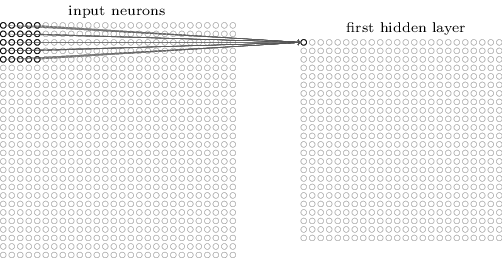
\includegraphics{tikz44.png}
\caption{Figura 1: Redes Convolucionais}
\end{figure}

Isto torna particularmente interessante seu uso para imagens. Onde as
unidades de entradas são representadas pela intensidade dos pixels, e
no caso de imagens coloridas são acrescidas outras dimensões às
unidades de entrada.

Os pesos que mapeiam as unidades de entrada para as de saída são
matrizes que são chamadas de filtros, máscaras ou kernels. É possível
modificar alguns parâmetros das camadas como o \emph{stride}, passo que
o filtro dá ao fazer o mapeamento, o \emph{padding}, preenchimento que
aumenta o tamanho das bordas da camada de entrada com 0's e 1's. Além
disso é possível ter um filtro com mais de uma dimensão. Através desses
parâmetros é possível definir qual será o tamanho da camada de saída.

\begin{figure}[ht]
\centering
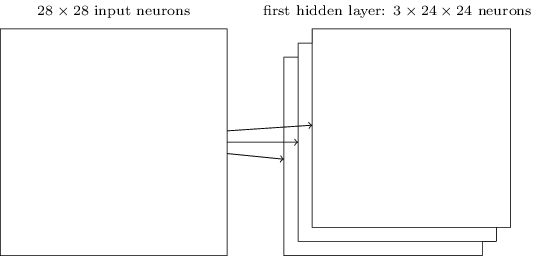
\includegraphics{tikz46.png}
\caption{Figura 2: Os filtros em uma rede convolucional}
\end{figure}

        \subsection{Batch Normalization}\label{batch-normalization}

\textbf{Batch Normalization}[4] é uma técnica de normalização de atributos que atua
entre as camadas convolucionais. A idéia é fazer com que as entradas de qualquer
camada tenha média zero e variância unitária, entretanto, esses parâmetros
(média e variância) podem ser alterados.

\begin{figure}[ht]
\centering
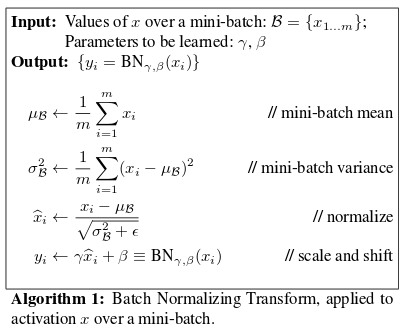
\includegraphics{batch_normalization_algorithm.png}
\caption{Algoritmo do Batch Normalization}
\end{figure}


A técnica de \textbf{Batch Normalization} permite que cada camada possa aprender
um pouco mais, por si mesma, independentemente das outras camadas.

    \section{Arquitetura Inicial}\label{arquitetura-inicial}

O projeto foi fortemente baseado no tutorial disponível em
\href{http://adventuresinmachinelearning.com/keras-tutorial-cnn-11-lines/}{[1]} sobre \textbf{Redes
Convolucionais} utilizando o \href{https://keras.io/}{keras}, e, portanto, inicialmente a
arquitetura utilizada foi a mesma sugerida no post, conforme a figura 3.

\begin{figure}[ht]
\centering
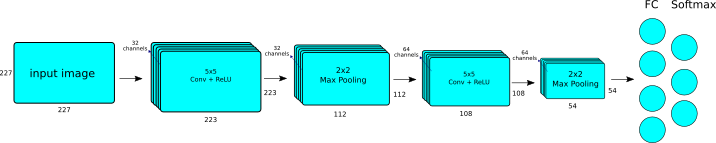
\includegraphics{arch-01.png}
\caption{Figura 3: Arquitetura Inicial}
\end{figure}


    \subsection{Projeto:}\label{projeto}

O nosso projeto consistiu em fazer um sistema de reconhecimento de peças
de xadres baseado em imagens já segmentadas. Dessa maneira utilizamos o
conjunto de dados(imagens) disponível em:
\href{https://www.dropbox.com/s/618l4ddoykotmru/Chess\%20ID\%20Public\%20Data.zip?dl=0}{
https://www.dropbox.com/s/618l4ddoykotmru/Chess ID Public Data.zip?dl=0}

Para fazer o projeto cogitamos inicialmente implementar o código na
biblioteca Tensorflow, porém por comodidade decidimos implementar na
biblioteca Keras por ser muito mais prático e intuitivo.

O primeiro passo foi fazer um \textbf{data augmentation} no dataset de
testes fazendo uma rotação nas imagens em 90, 180 e 270 graus,
triplicando o número de amostras, além de converter as imagens
\textbf{RGB} para \textbf{grayscale}, já que, pelo menos no xadrez
oficial, as peças só podem ser pretas ou brancas. Para isso foi
elaborado um script Python utilizando a biblioteca \textbf{OpenCV}. Após
feito o aumento dos dados foram criadas também algumas funções de forma
que as imagens fossem amostradas aleatóriamente para o conjunto de
treinamento e testes.

Assim já poderiamos começar o treinamento, o problema que nos deparamos
foi o de que não possuiamos GPU e como o conjunto de dados era muito
grande o tempo estimado para treinamento estava em mais de 30 horas.
Após uma pesquisa resolvemos utilizar o \textbf{Google Colab}[3] e seu
serviço de utilização de GPU remota, o que reduziu o tempo de
treinamento para \textbf{10 minutos} utilizando a mesma arquitetura
inicial.

A rede que usamos não teve um resultado tão bom inicialmente, atingindo uma
acurácia de aproximadamente \textbf{26\%}, então tomamos a decisão de tornar a
rede mais profunda. Feito isso a rede teve uma melhora significativa.
Finalmente tentamos diversas técnicas diferentes com o intuito de ter um aumento
significativo, onde observamos aumentos pequenos na performance com algumas
técnicas bem sucedidas e outras técnicas resultaram em uma piora considerável.

O melhor desempenho se deu ao incluirmos o \textbf{Batch Normalization} entre as
camadas, entretanto não podíamos dizer que a melhora do desempenho foi devido a
introdução do \textbf{Batch Normalization} pois não estávamos
\emph{"normalizando"} a geração dos números aleatórios, de forma que a
melhora pode ter sido proviniente de uma inicialização da rede com pesos
melhores.

Para termos uma certa garantia que a melhora do desempenho era devido as
modificações na arquitetura da rede, bem como introdução de regulação,
etc, adicionamos o seguinte código:

\begin{lstlisting}[language=Python]
# Algumas configurações para obter "resultados reproduzíveis"
np.random.seed(42)
rn.seed(54321)
session_config = tf.ConfigProto(
    intra_op_parallelism_threads=1,
    inter_op_parallelism_threads=1
)
tf.set_random_seed(1234)
sess = tf.Session(graph=tf.get_default_graph(), config=session_config)
keras.backend.set_session(sess)
\end{lstlisting}

Assim, com a melhor acurácia em torno de \textbf{69\%}, a solução
foi, a partir da arquitetura inicial, aprofundar a rede em mais camadas,
adicionando o \textbf{Batch Normalization} entre as camadas, de forma
que a arquitetura final ficou com 5 camadas \textbf{convolutivas} +
\textbf{max pooling} + \textbf{batch normalization} + 1 camada
\textbf{fully connected} com saída \textbf{softmax}. No treinamento
iniciamos com 10 épocas, mas vimos que ao aumentar o número de épocas, o
desempenho melhorava, mas como isso também aumentava o tempo de
treinamento, deixamos o treinamento com 20 épocas na fase final.

    \subsection{Resultados:}\label{resultados}

    Utilizando a arquitetura inicial, rodando 10 épocas, obtivemos uma acurácia de \textbf{50\%}.

\begin{figure}[ht]
\centering
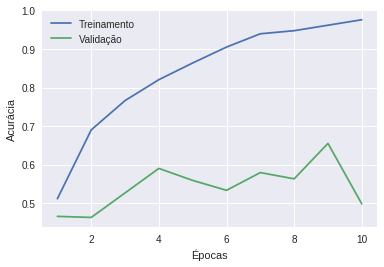
\includegraphics{acc-01.png}
\caption{Figura 4: Arquitetura inicial com 10 épocas, 50\% de acurácia}
\end{figure}

Após alguma modificações na rede e introduzindo \textbf{Batch Normalization}, a acurácia subiu para
\textbf{68\%}, conforme visto na figura 5.

\begin{figure}[ht]
\centering
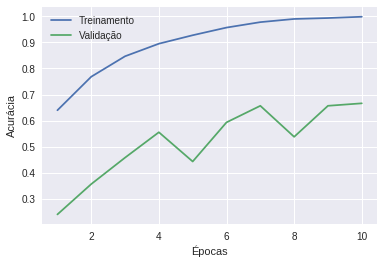
\includegraphics{acc-02-batch_n.png}
\caption{Figura 5: Adicionado o Batch Normalization}
\end{figure}


Assim, após mais alguns testes, aumentando o número de épocas para 20,
chegamos a uma acurácia de \textbf{69,46\%}, vide figura 6.

\begin{figure}[H]
\centering
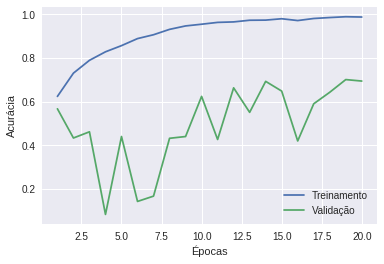
\includegraphics{acc6946-padding_same.png}
\caption{Figura 6: Arquitetura Final com 20 épocas, 69,46\% de acurácia}
\end{figure}


    \subsection{Conclusão:}\label{conclusao}

Durante o processo de adequação da rede, percebemos que, enquanto não \emph{"normalizamos"}
a geração dos números aleatórios, estava bem complicado construir uma arquitetura
que fosse satisfatória, pois ao treinar a mesma arquitetura mais de uma vez, obtínhamos
resultados bem diferentes, então, esse foi um passo importante no projeto para que
pudéssemos obter resultados mais consistentes e que refletiam as modificações que
estávamos fazendo na arquitetura da rede.

Também podemos comprovar que quanto mais profunda a rede, quanto mais camadas convolutivas
são acrescentadas à rede, isso reflete de maneira significativa no desempenho da mesma,
assim como aumenta significativamente o tempo de processamento.

Ainda há espaço para melhoramentos no projeto, como a inclusão de \emph{"Regulação"}, pois
percebemos que com o passar das \emph{épocas}, a rede vai aprendendo muito bem o conjunto
de treinamento mas não tem o mesmo desempenho suave no conjunto de testes.

    % Add a bibliography block to the postdoc

    \section{Referências:}\label{referencias}

[1] Tutorial Redes Convolucionais utilizando
Keras:
\href{http://adventuresinmachinelearning.com/keras-tutorial-cnn-11-lines/}{
http://adventuresinmachinelearning.com/keras-tutorial-cnn-11-lines/}\\

[2] Neural Networks and Deep Learning, Michael Nielsen:
\href{http://neuralnetworksanddeeplearning.com/}{http://neuralnetworksanddeeplearning.com/}\\

[3] Google Colab:
\href{https://colab.research.google.com}{https://colab.research.google.com}\\

[4] Ioffe, Sergey and Christian Szegedy. “Batch Normalization: Accelerating Deep Network Training by Reducing Internal Covariate Shift.” ICML (2015).

    \end{document}
